\chapter{Testing}
\label{ch:testing}

Diese Kapitel beschäftigt sich mit dem Prozess des Testens in diesem Projekt. Dabei soll zunächst wird etwas Theorie vorgestellt, in der klar gemacht werden soll, was Testen eigentlich ist, wie der Test Prozess im Projekt nach SCRUM gelebt wurde und welche Aufgaben dem Tester zufallen. Abgeschlossen wird dieses Kapitel dem beispielhaften Aufzeigen der Umsetzung der definierten Testmethoden in diesem Projekt.

\section{Definition Testen}
\label{sec:DefTest}

Softwaresysteme sind ein wesentlicher Bestandteil des Lebens: von Fachanwendungen (z.B. im Bankwesen) bis hin zu Verbraucherprodukten (z.B. Autos). Die meisten Menschen haben bereits Erfahrungen mit Software gemacht, die nicht wie erwartet funktioniert hat. Software, die nicht korrekt arbeitet, kann zu vielfältigen Problemen führen, u.a. zu Geld-, Zeit- oder Imageverlust, sogar bis hin zu Verletzungen oder Tod.
Softwaretesten ist ein Mittel, die Qualität von Software zu beurteilen und das Risiko einer Fehlerwirkung im Betrieb zu reduzieren.
Es ist eine gängige Fehleinschätzung, dass Testen ausschließlich darin besteht, Tests auszuführen, d.h. im Sinne von: die Software auszuführen und die Ergebnisse zu prüfen. Softwaretesten ist ein Prozess, der viele unterschiedliche Aktivitäten umfasst. Testen beinhaltet also auch die Prüfung von Arbeitsergebnissen wie Anforderungen, User-Stories und Quellcode im Rahmen von Reviews. Eine weitere gängige Fehleinschätzung ist, dass sich Testen ausschließlich auf die Verifizierung von Anforderungen, User-Stories oder anderen Spezifikationen konzentriert. Auch wenn das Testen es erfordert, zu prüfen, ob das System spezifische Anforderungen erfüllt, so umfasst es auch die Validierung, also die Prüfung, ob das System in seiner Einsatzumgebung die Bedürfnisse von Benutzern und anderen Stakeholdern erfüllen wird.

\section{Aufgabengebiet als Tester}
\label{sec:AufgTest}

Das Testen ist untrennbar mit der Entwicklung verwoben. Teammitglieder mit Testfokus decken mehrere Rollen ab: zum einen, die des Testers (operative Aufgaben), zum anderen die des Testmanagers (Strategische Aufgaben) und schließlich auch die des Qualitätsmanagers.

Jedes agile Team besteht aus zumindest ein bis zwei ausgebildete Tester. Weiterhin stehen dem Team ergänzend noch einige Support-Teams oder auch einzelne Fachexperten zur Verfügung, die für Spezialthemen herangezogen werden können (s. \autoref{fig:AufgGebietTester}).

\begin{figure}[!htb]
    \centering
    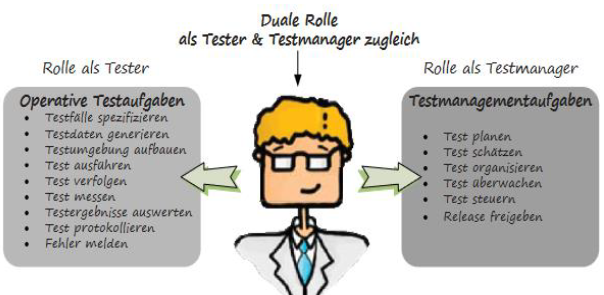
\includegraphics[width=.9\textwidth]{figures/rebecca/Aufgaben_Tester.png}
    \caption[]{Aufgabengebiete des Testers}
    \label{fig:AufgGebietTester}
\end{figure}

Vereinfacht kann die Teamzusammenstellung wie folgt dargestellt werden (\autoref{fig:team_position_tester}).

\begin{figure}[!htb]
    \centering
    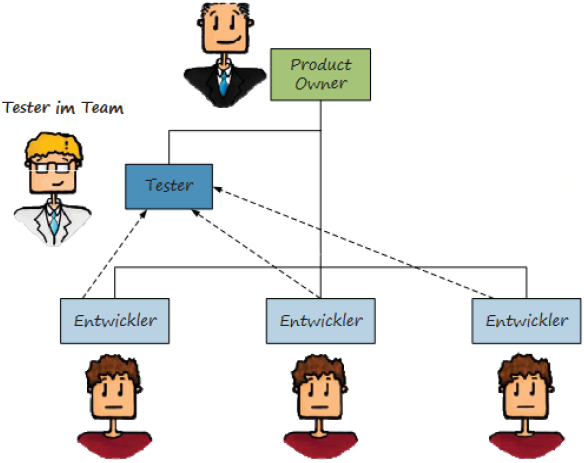
\includegraphics[width=.9\textwidth]{figures/rebecca/Position_Tester.png}
    \caption[]{Teamzusammenstellung und Position der Tester}
    \label{fig:team_position_tester}
\end{figure}

\section{Testen im agilen Projekt}
\label{sec:testen_agil}

Das Testen hat auch in SCRUM einen hohen Stellenwert. Die Rolle des Testers sollte ein fester Bestandteil eines cross-funktionalen Teams, die Qualitätssicherung automatisch in jedem Entwicklungszyklus integriert sein. Das agile Testen im SCRUM muss so gestaltet sein, dass es die Ziele der agilen Entwicklung unterstützt. Das heißt, es muss auf hohe Kundenzufriedenheit, hohe Produktivität und hohe Entwicklungsgeschwindigkeit ausgerichtet sein. Es muss schnell auf Änderungen reagieren können und selbstorganisiert sein.
Als agiles Testen wird das Testen von Software im Rahmen eines agilen Entwicklungsprojekts bezeichnet. Testen in agilen Entwicklungsprojekten bedarf dabei vor allem eines Fokus auf die Unterstützung des Entwicklungsteams.


\subsection{Wann in Scrum Testen}
\label{sub:WannTestenScrum}

Es gilt der Grundsatz von Realisierung und Test non-stop. Während des Sprints muss dafür gesorgt werden, dass die „Tester“ vom ersten Tag an ins Team integriert sind und parallel mit (bzw. zusammen mit) den „Entwicklern“ an der Realisierung der Stories arbeiten. Schlüsselfertigkeiten hierfür sind:

\begin{itemize}
    \item Die Beteiligung der Tester an der Sprint-Planung und den Weekly Scrum Meetings
    \item Die zeitliche Verschränkung von Entwicklungs- und Testaktivitäten. Hierzu sind Prinzipien wie „Test Driven Development“ bzw. „Test First“ und Pairing zwischen Entwicklern und Testern geeignet
    \item Die Kombination von systematischen Tests und explorativen Tests. Letztere liefern besonders schnell Feedback und finden Fehler, die von systematischen Tests ggf. nicht gefunden werden können. Diese wurden von mir als Tester durchgeführt.
    \item Die transparente Repräsentation von Tests in der Planung und Statusverfolgung durch geeignete Darstellung auf dem Taskboard, dem zentralen Planungsmittel des agilen Teams
\end{itemize}

\begin{figure}[!htb]
    \centering
    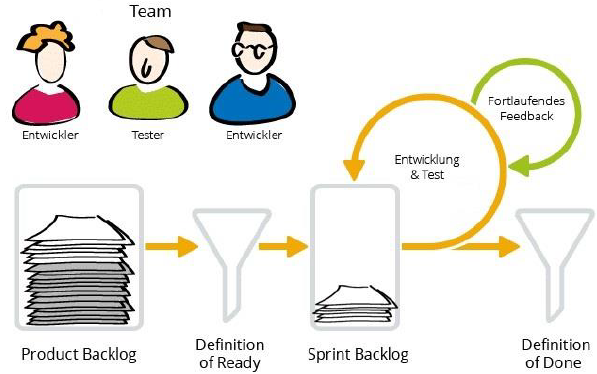
\includegraphics[width=.9\textwidth]{figures/rebecca/Wann_In_Scrum_Testen.png}
    \caption[]{Wann in Scrum Testen}
    \label{fig:WannTesten}
\end{figure}

\section{Test-Prozess}
\label{sec:TestProzess}

Der fundamentale Testprozess (FTP) ist einer der am verbreitetsten Testprozesse und mittlerweile internationaler ISTQB-Standard. Der Prozess beinhaltet verschiedene Testaktivitäten, welche während des gesamten Testprozesses abgedeckt sein sollten. Diese Aktivitäten sind die Testplanung, der Testentwurf, die anschließende Testimplementierung sowie deren Ausführung, eine anschließende Testauswertung sowie ein abschließender Testabschluss. Jeder der im Folgenden erklärten Testtypen (Entwicklertest, Inkrement Test und Release-Test) soll all diese Testaktivitäten strukturiert in unterschiedlicher Intensität anwenden. Die Testplanung findet während des Sprint-Plannings und des Daily Scrums (weekly), der Testentwurf, die Testimplementierung und -ausführung während des Sprints, die Testauswertung während des Sprint-Reviews sowie der Testabschluss während der Sprint-Retrospektive stattfinden sollen. Für die einzelnen Testaktivitäten in den jeweiligen Testtypen sollten die folgenden Aspekte genutzt werden: eine Testbasis, gegen welche getestet wird (z.B. Anforderungen im Backlog), die Testobjekte, welche getestet werden (z. B. ein Inkrement), die Teststufen und Testarten, welche durchgeführt werden (z. B. Systemtest als Teststufe und Regressionstest als Testart) sowie die verschiedenen Testwerkzeuge, welche das Testen unterstützen. (s. \autoref{fig:TestProzessBild})

\begin{figure}[!htb]
    \centering
    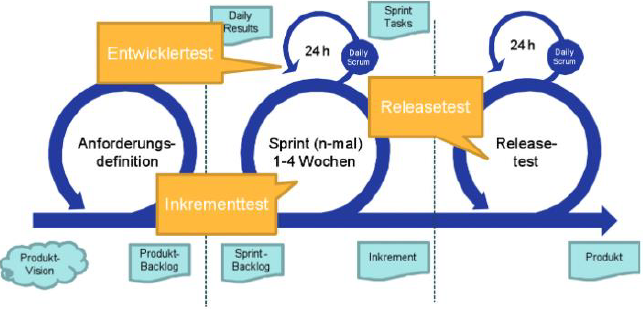
\includegraphics[width=.9\textwidth]{figures/rebecca/Testprozess.png}
    \caption[]{Testprozess}
    \label{fig:TestProzessBild}
\end{figure}

\subsection{Entwicklertest}
\label{sub:EntwicklerTest}

Der Entwicklertest findet während der täglichen (in diesem Projekt wöchentlichen) Entwicklungsarbeit statt. Das Test Ziel ist die Validierung der täglichen (wöchentlichen) Entwicklungsergebnisse gegen die Sprint-Tasks. Jeder Entwickler kümmert sich um seine aktuellen Sprint-Tasks, welche hier als Testbasis dienen, aus der die Testfälle abgeleitet werden müssen. Das Daily Scrum findet wie üblich, es werden allerdings zusätzlich auch die Testaufgaben und Testfälle besprochen. Diese Tests (s. \autoref{fig:EntwicklerTest}) werden vom Entwickler übernommen.

\begin{figure}[!htb]
    \centering
    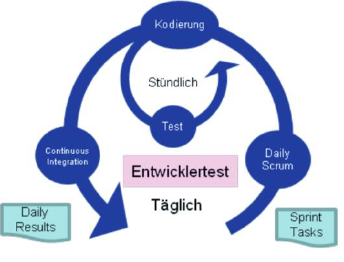
\includegraphics[width=.9\textwidth]{figures/rebecca/Entwickler_Test.png}
    \caption[]{Entwickler-Test}
    \label{fig:EntwicklerTest}
\end{figure}

\subsection{InkrementTest}
\label{sub:InkremenTest}

Der Entwicklertest findet im täglichen Rahmen statt, wohingegen der Inkrement-Test erst gegen Ende eines Sprints durchgeführt, wenn das Inkrement fertig wird. Obwohl Aktivitäten im Entwicklertest eine kontinuierliche Qualitätsüberwachung des Inkrements ermöglichen, ist am Ende eines Sprints ein dedizierter Inkrement-Test notwendig, um folgende Testziele zu gewährleisten.

\begin{itemize}
    \item Die korrekte Funktionsweise des im Sprint entwickelten Inkrements und des korrekten Zusammenspiels mit früher entwickelten Inkrementen soll gezeigt werden.
    \item Es soll sichergestellt werden, dass frühere Inkremente nicht verändert wurden. Der Test kann je nach Sprintlänge nach einer Woche oder auch erst nach vier Wochen durchgeführt
\end{itemize}

Gegen Ende des Sprints ist ein Regressionstest sehr wichtig ist, damit die alte Funktionalität immer noch richtig läuft, nachdem neue Funktionalität hinzugefügt wurde.
Die Testbasis sind im Gegensatz zum Entwicklertest nicht nur die einzelnen Sprint-Tasks, sondern das gesamte Sprint-Backlog, welches das zu liefernde Inkrement, hier auch das Testobjekt, definiert. Die Definition of Done besagt, wann ein Task wirklich fertig ist, wozu u. a. auch das Testen gehört. Im abschließenden Review Meeting, wird diese „Definition of Done“ vom Team zusammen mit dem Product Owner ausgewertet, ob sie für die Entwicklung und das Testen des Inkrements erfüllt wurde. Zur Testdurchführung gehören im Inkrement-Test als Teststufen neben dem Entwicklertest insbesondere auch der Systemtest, der prüft, ob das entsprechende Inkrement als ein Ganzes funktioniert und so vom Benutzer akzeptiert wird. Als Testarten gehören zu diesem Test-Typ nicht nur die funktionalen Tests und Regressionstests, sondern insbesondere auch die nicht-funktionalen Tests, wie beispielsweise Performanz Tests, Usability-Tests usw.

\begin{figure}[!htb]
    \centering
    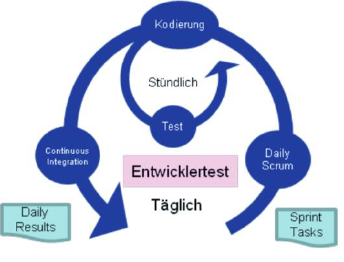
\includegraphics[width=.9\textwidth]{figures/rebecca/Inkrement_Test.png}
    \caption[]{Inkrement-Test}
    \label{fig:InkrementTest}
\end{figure}

\subsection{Release-Test}
\label{sub:release_test}

Der Release-Test wird das Produkt in seiner Gesamtheit getestet. Der Release-Test findet abschließend nach den Inkrementtests in Form eines dedizierten Sprints statt. Häufig wird eine Software inpotenziell fertigen Inkrementen entwickelt, welche aber anschließend zu einem gesamten Release zusammengefasst wird. Am Anfang wird geplant, nach wie vielen Sprints ein Release üblicherweise fertig sein soll. Der Release-Test kann nun ebenfalls als ein Sprint aufgebaut werden und ist damit weiter Scrum-Konform. Die Testbasis ist hier nun das gesamte Product Backlog, da hier nicht nur ein Inkrement nach einem Sprint, sondern das gesamte Produkt das Testobjekt ist. Anstatt eines Sprint-Backlogs kann analog ein sogenanntes Test-Backlog erstellt werden, welches die gesamten Release-Tests enthält.

\begin{figure}[!htb]
    \centering
    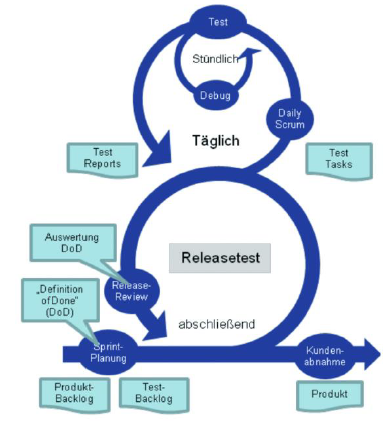
\includegraphics[width=.8\textwidth]{figures/rebecca/Release_Test.png}
    \caption[]{Release-Test}
    \label{fig:ReleaseTest}
\end{figure}

Als Teststufen enthalten diese Release-Tests Systemintegrationstests, Inbetriebnahmetests und insbesondere Akzeptanztests. Im Release-Test können die Testfälle aus den Inkrementtests wiederverwendet werden, sodass für den Testentwurf kein erheblicher Zusatzaufwand entsteht. Als Testart ist hier neben den funktionalen und nicht-funktionalen Tests auch das sogenannte End-To-End-Testing zu finden, welches über das gesamte System und Produkt im Zusammenspiel aller Komponenten stattfindet. Für die Durchführung der Tests wird das Test-Backlog analog zum Sprint-Backlog in Test-Tasks aufgeteilt, welche täglich entwickelt und durchgeführt werden. Weiterhin findet ein Daily Scrum statt um die Arbeit zu besprechen. Auf stündlicher Basis findet neben den Tests auch das Debugging statt, um Fehler zu finden und zu beheben. Am Ende des Tages steht ein Test-Report an. Am Ende des Sprints findet nicht nur eine Auswertung der speziellen Definition of Done bezüglich des Releases statt, sondern ebenfalls die finale Kundenabnahme des Produktes.


\section{Umsetzung im Projekt}
\label{sec:UmsetzungTest}

Hier soll nun genauer erläutert werden, welche der Testmethoden in dem Projekt genutzt wurden, um möglichste hohe fehlerfrei Qualität unsere Plattform zu gewährleisten.

\subsection{Testen gegen User-Stories}
\label{sub:UmsetzungTestGGUserStories}

Beim Abtesten der User-Stories wurde das Verfahren des Black-Box Testens angewandt. Bei einem Black-Box-Test werden die Testfälle ausschließlich aus der Spezifikation (User-Stories) des zu testenden Objekts abgeleitet, ohne dabei dessen innere Struktur, also Architektur und Code, zu berücksichtigen (- diese werden als „Black Box“ behandelt). Es wird also nur das von außen sichtbare Verhalten des Testobjektes beobachtet.

\begin{figure}[!htb]
    \centering
    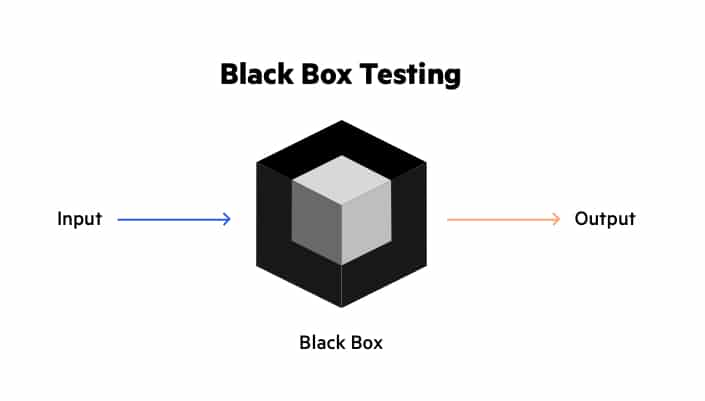
\includegraphics[width=.9\textwidth]{figures/rebecca/Black_Box_Testing.jpg}
    \caption[]{Black-Box-Testing}
    \label{fig:BlackBoxTest}
\end{figure}

Dabei wurde als Akzeptanzkriterium die Defintion of Done der einzelnen User Stories genutzt. Dabei wurde der Fokus auf das positive Testing und negative Testing gelegt. Zusätzlich wurden aber auch einige Grenzwert-Testfälle spezifiziert, wo dies nötig war, und durchgeführt.

\textbf{Positive Testing:} \\
Positivtests sind eine Art von Softwaretests, bei denen davon ausgegangen wird, dass alles so abläuft wie erwartet. Es wird mit der Annahme durchgeführt, dass nur gültige und relevante Dinge auftreten werden.

\textbf{Negative Testing:} \\
Negativtests sind eine Art von Softwaretests, die durchgeführt werden, um das System auf unerwartete Bedingungen zu prüfen. Negative Tests spielen eine wichtige Rolle bei der Entwicklung leistungsfähiger Software. Dabei wird geprüft, wie sich die Software unter solchen unerwarteten Bedingungen verhält.

\begin{figure}[!htb]
    \centering
    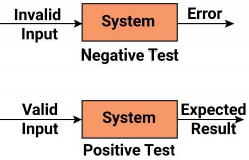
\includegraphics[width=.5\textwidth]{figures/rebecca/Neg_Pos_Testing.png}
    \caption[]{Negative vs. Positive Testing}
    \label{fig:negativ_vs_positiv_testing}
\end{figure}

\textbf{Grenzwert-Testing:} \\
Das Testen von Grenzwerten testet extreme Grenzen der Eingangswerte. Unter extreme Grenzen fal-len Enden wie Start-End-, Lower-Upper-, Maximum-Minimum-, Just Inside-Just Outside-Werte. Das Testen wird als 'Testen von Grenzwerten' bezeichnet.

\begin{figure}[!htb]
    \centering
    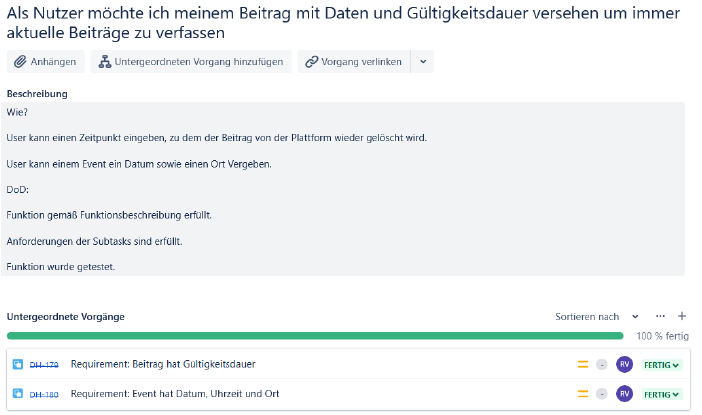
\includegraphics[width=.9\textwidth]{figures/rebecca/Beispiel_User_Story_Test.png}
    \caption[]{Beispiel User-Story für Test}
    \label{fig:BespielUserStory}
\end{figure}

Die Umsetzung soll nun im Folgenden anhand eines Beispiels genauer erklärt werden. In diesem Beispiel wird der Fokus nur auf die Angabe des Gültigkeitsdatums gelegt (DH-179).

\begin{figure}[!htb]
    \centering
    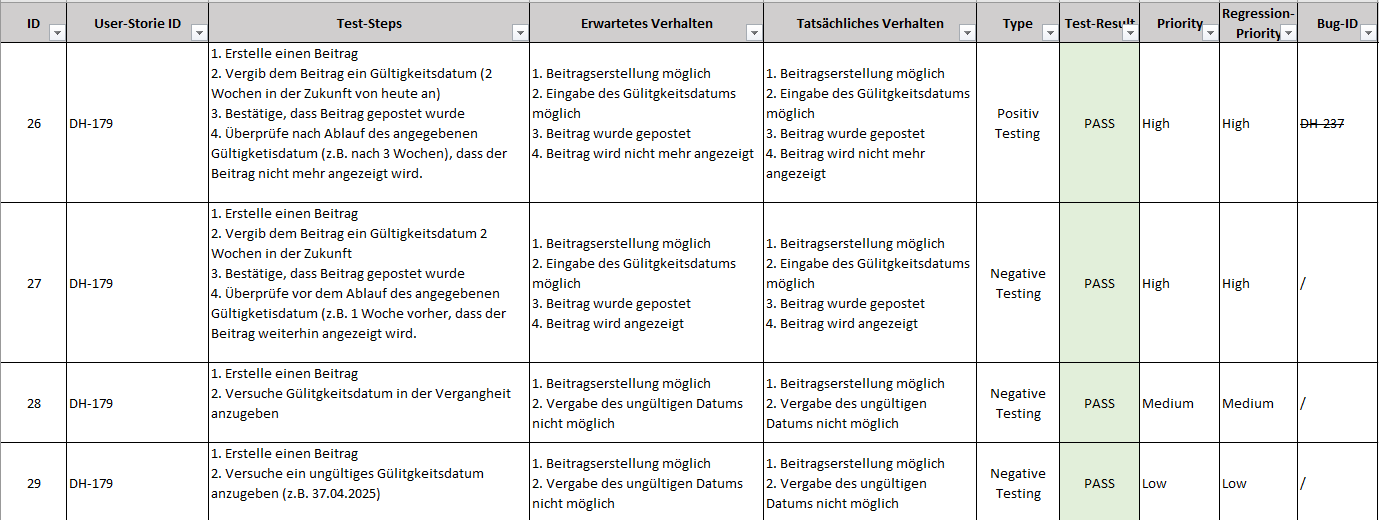
\includegraphics[width=.9\textwidth]{figures/rebecca/Umsetzung_Testfaelle}
    \caption[]{Umsetzung der Testfaelle}
    \label{fig:UmsetzungTestFaelle}
\end{figure}

\subsection{Regressions-Test}
\label{sub:UmsetzungTestRegression}

Wenn eine Software durch die Einführung neuer oder geänderter Funktionen an Funktionalität verliert, spricht man von einem Rückschritt zu einem weniger entwickelten Zustand. Selbst geringfügige Änderungen an der Software oder am ursprünglichen Code können zu erheblichen Fehlern wie Abstürzen, Störungen und teilweisem oder vollständigem Verlust der Funktionalität führen.
Regressionstests dienen dazu, diese Fehler zu erkennen und die Anwendung wieder zu stabilisieren. Sowohl funktionale als auch nicht-funktionale Testverfahren bewerten die Auswirkungen neuer Funktionen auf den bestehenden Code.
In diesem Projekt wurde das folgendermaßen gelebt: Die Testfälle gegen User-Stories (4.5.1) wurden priorisiert. Anschließend wurden 1-2 Testfälle ausgewählt zu jeder User-Story, welche nach einer Optimierung oder Änderung des dazugehörigen Feature jedes Mal mit ausgeführten wurden. Das bedeutet zum Beispiel, dass zunächst die Funktion des Beitrags erstellen möglich war. Anschließend wurde die Funktion des Gültigkeitsdatums hinzugefügt. Danach wurde überprüft, dass alle vorherigen Funktionen weiterhin die Defintion of Done erfüllen und alles weiterhin fehlerfrei funktioniert.
Eine vollständige Wiederholung aller Testfälle wurde im letzten Sprint vor dem Release vorgenommen (Release Test), um sicherzustellen, dass bei der Übergabe zum Kunden alles fehlerfrei funktioniert.

\begin{figure}[!htb]
    \centering
    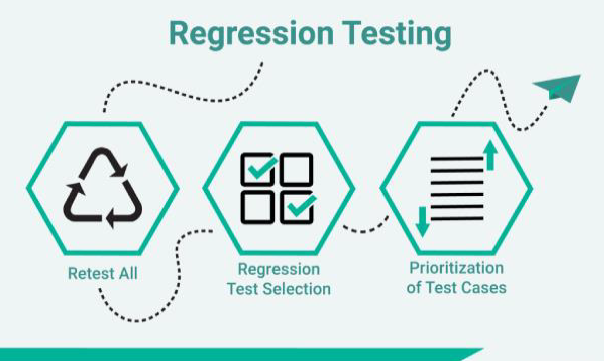
\includegraphics[width=.8\textwidth]{figures/rebecca/Regressions_Test.png}
    \caption[]{Regressions-Test}
    \label{fig:Regressionstest}
\end{figure}

\subsection{Feld-Test}
\label{sub:UmsetzungTestFeld}

Ein Feldtest ist die Erprobung einer produktionsfähigen Vorabversion einer Software durch eine repräsentative Anzahl an von Anwendern. Das Ziel eines Feldtests ist das Erkennen von noch nicht komplett spezifizierten Einsatzumgebungen und Bedingungen sowie dem Prüfen auf Akzeptanz des Marktes.
Dazu wurde eine bereite Anzahl an potentiellem Nutzer ins Visier genommen. Da die Plattform Generationenübergreifend sein soll, wurden daher Testpersonen mit unterschiedlichem Alter, unterschiedlichem Background Wissen und unterschiedlichen Interessen ausgewählt.
Für die Durchführung des Feld-Testes wurde eine Guideline erstellt und der Tester hat sich zusammen mit der Testperson an einen Rechner gesetzt und die aktuelle Plattform ausprobiert. Der Tester hat dabei die Testperson nur gebeten gewisse Aktionen durchzuführen und hat die Testperson gebeten, dabei unentwegt Rückmeldung darüber zu geben, welche Gefühle er dabei empfindet und wie ihm die bestehenden Features gefallen. Abgeschlossen wurde der Test dadurch, dass die Personen ein kurzes Feedback geben sollten.
Der Test wurde insgesamt drei Mal durchgeführt mit jeweils 6 Personen, und das Ergebnis wurde anschließend im Team besprochen, wo etwaige Änderungen vorgenommen werden müssen beziehungsweise welche Features eventuell neu priorisiert werden müssen.

\begin{figure}[!htb]
    \centering
    
\includegraphics[width=.8\textwidth]{figures/rebecca/Feld_Test_Konzept.png}
    \caption[]{Feld-Test}
    \label{fig:Feldtest}
\end{figure}

Teilnehmer:
\begin{itemize}
    \item P. Vogler (Alter: 53, weiblich, Bankkauffrau)
    \item N. Vogler (Alter: 55, männlich, Berufsschulehrer)
    \item D. Bandac (Alter: 26, männlich, Requirements-Ingenieur)
    \item D. Blana (Alter: 27, weiblich, Zahntechnikerin)
    \item T. Scholl (Alter: 36, männlich, System-Tester)
    \item K. Warmuth (Alter: 42, weiblich, Büro-Angestellte)
\end{itemize}

\subsection{Exploratives-Testen}
\label{sub:UmsetzungTestExplorativ}

Bei dieser Methode stehen nicht Testpläne im Mittelpunkt, sondern die Tester „entdecken“ die Anwendung schrittweise selbst, indem sie diese benutzen. Parallel dazu erstellen die ersten Testfälle und optimieren sie iterativ in dem Maße, in dem mehr über die Anwendung gelernt wird. Gefragt sind hierbei vor allen Dingen Intelligenz, Intuition und Erfahrung. Im Gegensatz zu den klassischen Testmethoden – die dadurch keineswegs obsolet werden – fokussiert sich der explorative Ansatz auf die grundsätzliche Benutzbarkeit der Anwendung. Denn Schwächen in der Darstellung, umständliche Arbeitsabläufe oder logische Brüche, werden oft erst im Nutzererlebnis offenbar.

\begin{figure}[!htb]
    \centering
    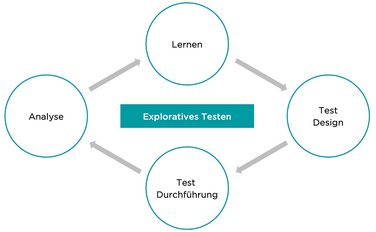
\includegraphics[width=.8\textwidth]{figures/rebecca/Exploratives_Testen.png}
    \caption[]{Exploratives Testen}
    \label{fig:explorativesTesten}
\end{figure}

Hierbei spezialisierte vor allem Ende des jeden Sprints fokussiert. Dabei wurde überprüft, welche neuen Funktionen implementiert wurden. Anschließend wurden diese in den Fokus genommen und mit den bisherigen Funktionen zusammen ausprobiert. Dabei werden auch bereits bestehende Testfälle optimiert und neue Testfälle hinzugefügt (s. Dazu 4.5.1). Hinzu kommt, dass dabei auch die Usability der einzelnen Funktionen überprüft wurden um die Qualität unserer Plattform aus der Sicht des Endbenutzers zu bewerten.
Bei Auffälligkeiten wurden im Weekly Meeting Rücksprache mit dem Team gehalten, um etwaige Änderungen am Design zu erörtern und in die Wireframes wenn nötig einzubinden.
Bei Fehlern wurde ein Fehlerbericht erstellt (Bug-Bericht), und dem jeweiligen Entwickler in Jira zugewiesen.